\documentclass[twoside]{book}

% Packages required by doxygen
\usepackage{calc}
\usepackage{doxygen}
\usepackage{graphicx}
\usepackage[utf8]{inputenc}
\usepackage{makeidx}
\usepackage{multicol}
\usepackage{multirow}
\usepackage{textcomp}
\usepackage[table]{xcolor}

% Font selection
\usepackage[T1]{fontenc}
\usepackage{mathptmx}
\usepackage[scaled=.90]{helvet}
\usepackage{courier}
\usepackage{amssymb}
\usepackage{sectsty}
\renewcommand{\familydefault}{\sfdefault}
\allsectionsfont{%
  \fontseries{bc}\selectfont%
  \color{darkgray}%
}
\renewcommand{\DoxyLabelFont}{%
  \fontseries{bc}\selectfont%
  \color{darkgray}%
}

% Page & text layout
\usepackage{geometry}
\geometry{%
  a4paper,%
  top=2.5cm,%
  bottom=2.5cm,%
  left=2.5cm,%
  right=2.5cm%
}
\tolerance=750
\hfuzz=15pt
\hbadness=750
\setlength{\emergencystretch}{15pt}
\setlength{\parindent}{0cm}
\setlength{\parskip}{0.2cm}
\makeatletter
\renewcommand{\paragraph}{%
  \@startsection{paragraph}{4}{0ex}{-1.0ex}{1.0ex}{%
    \normalfont\normalsize\bfseries\SS@parafont%
  }%
}
\renewcommand{\subparagraph}{%
  \@startsection{subparagraph}{5}{0ex}{-1.0ex}{1.0ex}{%
    \normalfont\normalsize\bfseries\SS@subparafont%
  }%
}
\makeatother

% Headers & footers
\usepackage{fancyhdr}
\pagestyle{fancyplain}
\fancyhead[LE]{\fancyplain{}{\bfseries\thepage}}
\fancyhead[CE]{\fancyplain{}{}}
\fancyhead[RE]{\fancyplain{}{\bfseries\leftmark}}
\fancyhead[LO]{\fancyplain{}{\bfseries\rightmark}}
\fancyhead[CO]{\fancyplain{}{}}
\fancyhead[RO]{\fancyplain{}{\bfseries\thepage}}
\fancyfoot[LE]{\fancyplain{}{}}
\fancyfoot[CE]{\fancyplain{}{}}
\fancyfoot[RE]{\fancyplain{}{\bfseries\scriptsize Generated on Tue Jun 11 2013 13:36:41 for Eco Sensor Pod by Doxygen }}
\fancyfoot[LO]{\fancyplain{}{\bfseries\scriptsize Generated on Tue Jun 11 2013 13:36:41 for Eco Sensor Pod by Doxygen }}
\fancyfoot[CO]{\fancyplain{}{}}
\fancyfoot[RO]{\fancyplain{}{}}
\renewcommand{\footrulewidth}{0.4pt}
\renewcommand{\chaptermark}[1]{%
  \markboth{#1}{}%
}
\renewcommand{\sectionmark}[1]{%
  \markright{\thesection\ #1}%
}

% Indices & bibliography
\usepackage{natbib}
\usepackage[titles]{tocloft}
\setcounter{tocdepth}{3}
\setcounter{secnumdepth}{5}
\makeindex

% Custom commands
\newcommand{\clearemptydoublepage}{%
  \newpage{\pagestyle{empty}\cleardoublepage}%
}


%===== C O N T E N T S =====

\begin{document}

% Titlepage & ToC
\pagenumbering{roman}
\begin{titlepage}
\vspace*{7cm}
\begin{center}%
{\Large Eco Sensor Pod }\\
\vspace*{1cm}
{\large Generated by Doxygen 1.8.4}\\
\vspace*{0.5cm}
{\small Tue Jun 11 2013 13:36:41}\\
\end{center}
\end{titlepage}
\clearemptydoublepage
\tableofcontents
\clearemptydoublepage
\pagenumbering{arabic}

%--- Begin generated contents ---
\chapter{bootstrap-\/notify}
\label{md_WebContent_bootstrap-notify-master_README}
Bootstrap alert system made better.

\section*{Copyright}

\begin{DoxyVerb}Copyright 2013 Nijiko Yonskai @nijikokun
Copyright 2012 Goodybag, Inc.
\end{DoxyVerb}


\section*{License}

Licensed under the Apache License, Version 2.\-0 (the \char`\"{}\-License\char`\"{}); you may not use this file except in compliance with the License. You may obtain a copy of the License at

{\tt http\-://www.\-apache.\-org/licenses/\-L\-I\-C\-E\-N\-S\-E-\/2.\-0}

Unless required by applicable law or agreed to in writing, software distributed under the License is distributed on an \char`\"{}\-A\-S I\-S\char`\"{} B\-A\-S\-I\-S, W\-I\-T\-H\-O\-U\-T W\-A\-R\-R\-A\-N\-T\-I\-E\-S O\-R C\-O\-N\-D\-I\-T\-I\-O\-N\-S O\-F A\-N\-Y K\-I\-N\-D, either express or implied. See the License for the specific language governing permissions and limitations under the License. 
\chapter{Namespace Index}
\section{Namespace List}
Here is a list of all namespaces with brief descriptions\-:\begin{DoxyCompactList}
\item\contentsline{section}{{\bf com} }{\pageref{namespacecom}}{}
\item\contentsline{section}{{\bf com.\-srccodes} }{\pageref{namespacecom_1_1srccodes}}{}
\item\contentsline{section}{{\bf com.\-srccodes.\-example} }{\pageref{namespacecom_1_1srccodes_1_1example}}{}
\end{DoxyCompactList}

\chapter{Hierarchical Index}
\section{Class Hierarchy}
This inheritance list is sorted roughly, but not completely, alphabetically\-:\begin{DoxyCompactList}
\item \contentsline{section}{com.\-srccodes.\-example.\-Sensor\-Data}{\pageref{classcom_1_1srccodes_1_1example_1_1_sensor_data}}{}
\item \contentsline{section}{com.\-srccodes.\-example.\-Sensor\-Data\-Retriever}{\pageref{classcom_1_1srccodes_1_1example_1_1_sensor_data_retriever}}{}
\item Http\-Servlet\begin{DoxyCompactList}
\item \contentsline{section}{com.\-srccodes.\-example.\-Data\-Facilitator}{\pageref{classcom_1_1srccodes_1_1example_1_1_data_facilitator}}{}
\end{DoxyCompactList}
\end{DoxyCompactList}

\chapter{Class Index}
\section{Class List}
Here are the classes, structs, unions and interfaces with brief descriptions\-:\begin{DoxyCompactList}
\item\contentsline{section}{{\bf com.\-srccodes.\-example.\-Data\-Facilitator} }{\pageref{classcom_1_1srccodes_1_1example_1_1_data_facilitator}}{}
\item\contentsline{section}{{\bf com.\-srccodes.\-example.\-Sensor\-Data} }{\pageref{classcom_1_1srccodes_1_1example_1_1_sensor_data}}{}
\item\contentsline{section}{{\bf com.\-srccodes.\-example.\-Sensor\-Data\-Retriever} }{\pageref{classcom_1_1srccodes_1_1example_1_1_sensor_data_retriever}}{}
\end{DoxyCompactList}

\chapter{File Index}
\section{File List}
Here is a list of all files with brief descriptions\-:\begin{DoxyCompactList}
\item\contentsline{section}{src/com/srccodes/example/{\bf Data\-Facilitator.\-java} }{\pageref{_data_facilitator_8java}}{}
\item\contentsline{section}{src/com/srccodes/example/{\bf Sensor\-Data.\-java} }{\pageref{_sensor_data_8java}}{}
\item\contentsline{section}{src/com/srccodes/example/{\bf Sensor\-Data\-Retriever.\-java} }{\pageref{_sensor_data_retriever_8java}}{}
\item\contentsline{section}{Web\-Content/{\bf Deprecated\-Draw.\-js} }{\pageref{_deprecated_draw_8js}}{}
\item\contentsline{section}{Web\-Content/{\bf draw.\-js} }{\pageref{draw_8js}}{}
\item\contentsline{section}{Web\-Content/assets/js/{\bf bootstrap.\-js} }{\pageref{bootstrap_8js}}{}
\item\contentsline{section}{Web\-Content/assets/js/{\bf bootstrap.\-min.\-js} }{\pageref{bootstrap_8min_8js}}{}
\item\contentsline{section}{Web\-Content/bootstrap-\/notify-\/master/js/{\bf bootstrap-\/notify.\-js} }{\pageref{bootstrap-notify_8js}}{}
\item\contentsline{section}{Web\-Content/datepicker/js/{\bf bootstrap-\/datepicker.\-js} }{\pageref{bootstrap-datepicker_8js}}{}
\end{DoxyCompactList}

\chapter{Namespace Documentation}
\section{Package com}
\label{namespacecom}\index{com@{com}}
\subsection*{Packages}
\begin{DoxyCompactItemize}
\item 
package {\bf srccodes}
\end{DoxyCompactItemize}

\section{Package com.\-srccodes}
\label{namespacecom_1_1srccodes}\index{com.\-srccodes@{com.\-srccodes}}
\subsection*{Packages}
\begin{DoxyCompactItemize}
\item 
package {\bf example}
\end{DoxyCompactItemize}

\section{Package com.\-srccodes.\-example}
\label{namespacecom_1_1srccodes_1_1example}\index{com.\-srccodes.\-example@{com.\-srccodes.\-example}}
\subsection*{Classes}
\begin{DoxyCompactItemize}
\item 
class {\bf Data\-Facilitator}
\item 
class {\bf Sensor\-Data}
\item 
class {\bf Sensor\-Data\-Retriever}
\end{DoxyCompactItemize}

\chapter{Class Documentation}
\section{com.\-srccodes.\-example.\-Data\-Facilitator Class Reference}
\label{classcom_1_1srccodes_1_1example_1_1_data_facilitator}\index{com.\-srccodes.\-example.\-Data\-Facilitator@{com.\-srccodes.\-example.\-Data\-Facilitator}}
Inheritance diagram for com.\-srccodes.\-example.\-Data\-Facilitator\-:\begin{figure}[H]
\begin{center}
\leavevmode
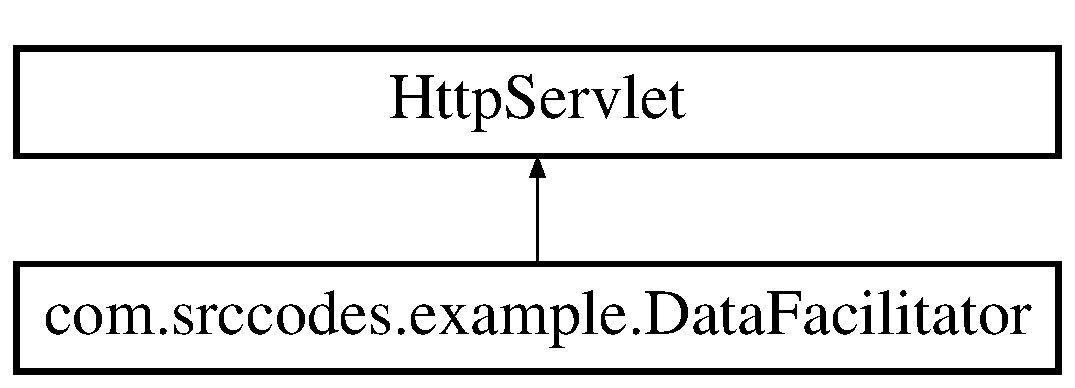
\includegraphics[height=2.000000cm]{classcom_1_1srccodes_1_1example_1_1_data_facilitator}
\end{center}
\end{figure}
\subsection*{Protected Member Functions}
\begin{DoxyCompactItemize}
\item 
void {\bf do\-Post} (Http\-Servlet\-Request request, Http\-Servlet\-Response response)  throws Servlet\-Exception, I\-O\-Exception 
\end{DoxyCompactItemize}
\subsection*{Static Private Attributes}
\begin{DoxyCompactItemize}
\item 
static final long {\bf serial\-Version\-U\-I\-D} = 1\-L
\end{DoxyCompactItemize}


\subsection{Detailed Description}
Servlet implementation class \doxyref{Data\-Facilitator}{p.}{classcom_1_1srccodes_1_1example_1_1_data_facilitator}

Purpose\-: The \char`\"{}\-M\-I\-D\-D\-L\-E-\/\-E\-N\-D\char`\"{}. Acts as the middle man between front and back end. Communicates requests and replies to and from each. Parses results into J\-S\-O\-N

Author\-: Michael Chamoures

Date\-: 6/11/2013 

\subsection{Member Function Documentation}
\index{com\-::srccodes\-::example\-::\-Data\-Facilitator@{com\-::srccodes\-::example\-::\-Data\-Facilitator}!do\-Post@{do\-Post}}
\index{do\-Post@{do\-Post}!com::srccodes::example::DataFacilitator@{com\-::srccodes\-::example\-::\-Data\-Facilitator}}
\subsubsection[{do\-Post}]{\setlength{\rightskip}{0pt plus 5cm}void com.\-srccodes.\-example.\-Data\-Facilitator.\-do\-Post (
\begin{DoxyParamCaption}
\item[{Http\-Servlet\-Request}]{request, }
\item[{Http\-Servlet\-Response}]{response}
\end{DoxyParamCaption}
) throws Servlet\-Exception, I\-O\-Exception\hspace{0.3cm}{\ttfamily [inline]}, {\ttfamily [protected]}}\label{classcom_1_1srccodes_1_1example_1_1_data_facilitator_a482e499501f40c3af8324ecf170d3929}
Intercepts J\-Query/\-A\-J\-A\-X Post() requests from the front-\/end \doxyref{draw.\-js}{p.}{draw_8js} 
\begin{DoxyParams}{Parameters}
{\em request} & The various request variables passed from \doxyref{draw.\-js}{p.}{draw_8js} \\
\hline
{\em response} & Used to write back the J\-S\-O\-N response to the front-\/end to be charted \\
\hline
\end{DoxyParams}


\subsection{Member Data Documentation}
\index{com\-::srccodes\-::example\-::\-Data\-Facilitator@{com\-::srccodes\-::example\-::\-Data\-Facilitator}!serial\-Version\-U\-I\-D@{serial\-Version\-U\-I\-D}}
\index{serial\-Version\-U\-I\-D@{serial\-Version\-U\-I\-D}!com::srccodes::example::DataFacilitator@{com\-::srccodes\-::example\-::\-Data\-Facilitator}}
\subsubsection[{serial\-Version\-U\-I\-D}]{\setlength{\rightskip}{0pt plus 5cm}final long com.\-srccodes.\-example.\-Data\-Facilitator.\-serial\-Version\-U\-I\-D = 1\-L\hspace{0.3cm}{\ttfamily [static]}, {\ttfamily [private]}}\label{classcom_1_1srccodes_1_1example_1_1_data_facilitator_a4fd75010caeac902b71ca30cad8bfa69}


The documentation for this class was generated from the following file\-:\begin{DoxyCompactItemize}
\item 
src/com/srccodes/example/{\bf Data\-Facilitator.\-java}\end{DoxyCompactItemize}

\section{com.\-srccodes.\-example.\-Sensor\-Data Class Reference}
\label{classcom_1_1srccodes_1_1example_1_1_sensor_data}\index{com.\-srccodes.\-example.\-Sensor\-Data@{com.\-srccodes.\-example.\-Sensor\-Data}}
\subsection*{Public Member Functions}
\begin{DoxyCompactItemize}
\item 
{\bf Sensor\-Data} ()
\item 
{\bf Sensor\-Data} (int num\-Units)
\item 
double[$\,$] {\bf get\-Data} ()
\item 
double[$\,$] {\bf get\-Time\-Stamp} ()
\item 
void {\bf set\-Data} (double[$\,$] {\bf new\-Data})
\item 
void {\bf set\-Time\-Stamp} (double[$\,$] {\bf time\-Stamp})
\end{DoxyCompactItemize}
\subsection*{Public Attributes}
\begin{DoxyCompactItemize}
\item 
double[$\,$] {\bf data}
\item 
double[$\,$] {\bf time\-Stamp}
\end{DoxyCompactItemize}


\subsection{Detailed Description}
\doxyref{Sensor\-Data}{p.}{classcom_1_1srccodes_1_1example_1_1_sensor_data} Class

Created 2/17/2013 by Michael Chamoures

Purpose\-: Each object represents a type of Sensor Data (i.\-e. wind direction, ph, etc.) Contains a double type value for the sensor reading itself, and a double value for representing the time\-Stamp of that data 

\subsection{Constructor \& Destructor Documentation}
\index{com\-::srccodes\-::example\-::\-Sensor\-Data@{com\-::srccodes\-::example\-::\-Sensor\-Data}!Sensor\-Data@{Sensor\-Data}}
\index{Sensor\-Data@{Sensor\-Data}!com::srccodes::example::SensorData@{com\-::srccodes\-::example\-::\-Sensor\-Data}}
\subsubsection[{Sensor\-Data}]{\setlength{\rightskip}{0pt plus 5cm}com.\-srccodes.\-example.\-Sensor\-Data.\-Sensor\-Data (
\begin{DoxyParamCaption}
{}
\end{DoxyParamCaption}
)\hspace{0.3cm}{\ttfamily [inline]}}\label{classcom_1_1srccodes_1_1example_1_1_sensor_data_a313efaace7261cecc2973d345f889568}
Constructor Defaults to initialize each array to length 1 \index{com\-::srccodes\-::example\-::\-Sensor\-Data@{com\-::srccodes\-::example\-::\-Sensor\-Data}!Sensor\-Data@{Sensor\-Data}}
\index{Sensor\-Data@{Sensor\-Data}!com::srccodes::example::SensorData@{com\-::srccodes\-::example\-::\-Sensor\-Data}}
\subsubsection[{Sensor\-Data}]{\setlength{\rightskip}{0pt plus 5cm}com.\-srccodes.\-example.\-Sensor\-Data.\-Sensor\-Data (
\begin{DoxyParamCaption}
\item[{int}]{num\-Units}
\end{DoxyParamCaption}
)\hspace{0.3cm}{\ttfamily [inline]}}\label{classcom_1_1srccodes_1_1example_1_1_sensor_data_a7146505ea42f00b019f9a5e158950588}
Constructor Defaults to initialize each array to length 1 
\begin{DoxyParams}{Parameters}
{\em num\-Unites} & Length to initialize instance variable arrays \\
\hline
\end{DoxyParams}


\subsection{Member Function Documentation}
\index{com\-::srccodes\-::example\-::\-Sensor\-Data@{com\-::srccodes\-::example\-::\-Sensor\-Data}!get\-Data@{get\-Data}}
\index{get\-Data@{get\-Data}!com::srccodes::example::SensorData@{com\-::srccodes\-::example\-::\-Sensor\-Data}}
\subsubsection[{get\-Data}]{\setlength{\rightskip}{0pt plus 5cm}double [$\,$] com.\-srccodes.\-example.\-Sensor\-Data.\-get\-Data (
\begin{DoxyParamCaption}
{}
\end{DoxyParamCaption}
)\hspace{0.3cm}{\ttfamily [inline]}}\label{classcom_1_1srccodes_1_1example_1_1_sensor_data_a9c2d02a88e70a1a587d7fd9805533fec}
\begin{DoxyReturn}{Returns}
Obect's current data array 
\end{DoxyReturn}
\index{com\-::srccodes\-::example\-::\-Sensor\-Data@{com\-::srccodes\-::example\-::\-Sensor\-Data}!get\-Time\-Stamp@{get\-Time\-Stamp}}
\index{get\-Time\-Stamp@{get\-Time\-Stamp}!com::srccodes::example::SensorData@{com\-::srccodes\-::example\-::\-Sensor\-Data}}
\subsubsection[{get\-Time\-Stamp}]{\setlength{\rightskip}{0pt plus 5cm}double [$\,$] com.\-srccodes.\-example.\-Sensor\-Data.\-get\-Time\-Stamp (
\begin{DoxyParamCaption}
{}
\end{DoxyParamCaption}
)\hspace{0.3cm}{\ttfamily [inline]}}\label{classcom_1_1srccodes_1_1example_1_1_sensor_data_aecb6406ea8b0ce2ecf110810d3330fa3}
\begin{DoxyReturn}{Returns}
Obect's current timestamp array 
\end{DoxyReturn}
\index{com\-::srccodes\-::example\-::\-Sensor\-Data@{com\-::srccodes\-::example\-::\-Sensor\-Data}!set\-Data@{set\-Data}}
\index{set\-Data@{set\-Data}!com::srccodes::example::SensorData@{com\-::srccodes\-::example\-::\-Sensor\-Data}}
\subsubsection[{set\-Data}]{\setlength{\rightskip}{0pt plus 5cm}void com.\-srccodes.\-example.\-Sensor\-Data.\-set\-Data (
\begin{DoxyParamCaption}
\item[{double[$\,$]}]{new\-Data}
\end{DoxyParamCaption}
)\hspace{0.3cm}{\ttfamily [inline]}}\label{classcom_1_1srccodes_1_1example_1_1_sensor_data_a13daa34908bb8fef90af38a4aa47eb2a}

\begin{DoxyParams}{Parameters}
{\em new\-Data} & Newly fetched data to fill data instance with \\
\hline
\end{DoxyParams}
\index{com\-::srccodes\-::example\-::\-Sensor\-Data@{com\-::srccodes\-::example\-::\-Sensor\-Data}!set\-Time\-Stamp@{set\-Time\-Stamp}}
\index{set\-Time\-Stamp@{set\-Time\-Stamp}!com::srccodes::example::SensorData@{com\-::srccodes\-::example\-::\-Sensor\-Data}}
\subsubsection[{set\-Time\-Stamp}]{\setlength{\rightskip}{0pt plus 5cm}void com.\-srccodes.\-example.\-Sensor\-Data.\-set\-Time\-Stamp (
\begin{DoxyParamCaption}
\item[{double[$\,$]}]{time\-Stamp}
\end{DoxyParamCaption}
)\hspace{0.3cm}{\ttfamily [inline]}}\label{classcom_1_1srccodes_1_1example_1_1_sensor_data_a269b11527fc5b2a069faee7a2f33b4c6}

\begin{DoxyParams}{Parameters}
{\em new\-Data} & Newly fetched data to fill timestamp instance with \\
\hline
\end{DoxyParams}


\subsection{Member Data Documentation}
\index{com\-::srccodes\-::example\-::\-Sensor\-Data@{com\-::srccodes\-::example\-::\-Sensor\-Data}!data@{data}}
\index{data@{data}!com::srccodes::example::SensorData@{com\-::srccodes\-::example\-::\-Sensor\-Data}}
\subsubsection[{data}]{\setlength{\rightskip}{0pt plus 5cm}double [$\,$] com.\-srccodes.\-example.\-Sensor\-Data.\-data}\label{classcom_1_1srccodes_1_1example_1_1_sensor_data_adf1a5318da81934776a2c3e6e0151fb1}
Data array for a sensors fetched data \index{com\-::srccodes\-::example\-::\-Sensor\-Data@{com\-::srccodes\-::example\-::\-Sensor\-Data}!time\-Stamp@{time\-Stamp}}
\index{time\-Stamp@{time\-Stamp}!com::srccodes::example::SensorData@{com\-::srccodes\-::example\-::\-Sensor\-Data}}
\subsubsection[{time\-Stamp}]{\setlength{\rightskip}{0pt plus 5cm}double [$\,$] com.\-srccodes.\-example.\-Sensor\-Data.\-time\-Stamp}\label{classcom_1_1srccodes_1_1example_1_1_sensor_data_a1796c2b4930646691752975f15b7bbb8}
Sec after 1970, jan 1st for each data pt 

The documentation for this class was generated from the following file\-:\begin{DoxyCompactItemize}
\item 
src/com/srccodes/example/{\bf Sensor\-Data.\-java}\end{DoxyCompactItemize}

\section{com.\-srccodes.\-example.\-Sensor\-Data\-Retriever Class Reference}
\label{classcom_1_1srccodes_1_1example_1_1_sensor_data_retriever}\index{com.\-srccodes.\-example.\-Sensor\-Data\-Retriever@{com.\-srccodes.\-example.\-Sensor\-Data\-Retriever}}
\subsection*{Public Member Functions}
\begin{DoxyCompactItemize}
\item 
{\bf Sensor\-Data\-Retriever} (String {\bf host\-Address}, String {\bf port\-Number})
\item 
{\bf Sensor\-Data\-Retriever} (String {\bf host\-Address}, String {\bf port\-Number}, String channel\-Name)  throws S\-A\-P\-I\-Exception
\item 
void {\bf go\-Fetch\-Data} (int start, int duration, String time\-Ref)  throws S\-A\-P\-I\-Exception 
\item 
void {\bf Reset\-Connection} (int {\bf units\-Per\-Fetch})
\item 
void {\bf End\-Connection} ()
\end{DoxyCompactItemize}
\subsection*{Public Attributes}
\begin{DoxyCompactItemize}
\item 
{\bf Sensor\-Data} {\bf sensor\-Data}
\item 
int {\bf requested\-Channel\-Index}
\item 
String[$\,$] {\bf channel\-Names}
\item 
int {\bf units\-Per\-Fetch}
\end{DoxyCompactItemize}
\subsection*{Private Attributes}
\begin{DoxyCompactItemize}
\item 
Channel\-Map {\bf r\-Map}
\item 
Sink {\bf sink}
\end{DoxyCompactItemize}


\subsection{Detailed Description}
B\-A\-C\-K\-E\-N\-D\-: \doxyref{Sensor\-Data\-Retriever}{p.}{classcom_1_1srccodes_1_1example_1_1_sensor_data_retriever} Class

Purpose\-: Contains all the Data\-Turbine retrieval tasks. Listens for requests from the \doxyref{Data\-Facilitator}{p.}{classcom_1_1srccodes_1_1example_1_1_data_facilitator} Servlet. Fetches data for the requested channel from the requested sensor pod deployment

Author\-: Michael Chamoures

Date\-: 6/11/2013 

\subsection{Constructor \& Destructor Documentation}
\index{com\-::srccodes\-::example\-::\-Sensor\-Data\-Retriever@{com\-::srccodes\-::example\-::\-Sensor\-Data\-Retriever}!Sensor\-Data\-Retriever@{Sensor\-Data\-Retriever}}
\index{Sensor\-Data\-Retriever@{Sensor\-Data\-Retriever}!com::srccodes::example::SensorDataRetriever@{com\-::srccodes\-::example\-::\-Sensor\-Data\-Retriever}}
\subsubsection[{Sensor\-Data\-Retriever}]{\setlength{\rightskip}{0pt plus 5cm}com.\-srccodes.\-example.\-Sensor\-Data\-Retriever.\-Sensor\-Data\-Retriever (
\begin{DoxyParamCaption}
\item[{String}]{host\-Address, }
\item[{String}]{port\-Number}
\end{DoxyParamCaption}
)\hspace{0.3cm}{\ttfamily [inline]}}\label{classcom_1_1srccodes_1_1example_1_1_sensor_data_retriever_a17ccfc12119b4fc68362a7e56e62bfb3}
Constructor. In the future this will be extended to construct a list of current available channel names. 
\begin{DoxyParams}{Parameters}
{\em host\-Address} & Host address of deployed sensor pod \\
\hline
{\em port\-Number} & Port number of deployed sensor pod \\
\hline
\end{DoxyParams}
\index{com\-::srccodes\-::example\-::\-Sensor\-Data\-Retriever@{com\-::srccodes\-::example\-::\-Sensor\-Data\-Retriever}!Sensor\-Data\-Retriever@{Sensor\-Data\-Retriever}}
\index{Sensor\-Data\-Retriever@{Sensor\-Data\-Retriever}!com::srccodes::example::SensorDataRetriever@{com\-::srccodes\-::example\-::\-Sensor\-Data\-Retriever}}
\subsubsection[{Sensor\-Data\-Retriever}]{\setlength{\rightskip}{0pt plus 5cm}com.\-srccodes.\-example.\-Sensor\-Data\-Retriever.\-Sensor\-Data\-Retriever (
\begin{DoxyParamCaption}
\item[{String}]{host\-Address, }
\item[{String}]{port\-Number, }
\item[{String}]{channel\-Name}
\end{DoxyParamCaption}
) throws S\-A\-P\-I\-Exception\hspace{0.3cm}{\ttfamily [inline]}}\label{classcom_1_1srccodes_1_1example_1_1_sensor_data_retriever_adf136882f72138b61a42165667b493ce}
Constructor if a channel name for a particular sensor is all that's requested.\-Opens a connection with the desired sensor pod and adds the channel\-Name to get data from to the channel map 
\begin{DoxyParams}{Parameters}
{\em host\-Address} & Host address of deployed sensor pod \\
\hline
{\em port\-Number} & Port number of deployed sensor pod \\
\hline
{\em channel\-Name} & Requested channel to get data from \\
\hline
\end{DoxyParams}


\subsection{Member Function Documentation}
\index{com\-::srccodes\-::example\-::\-Sensor\-Data\-Retriever@{com\-::srccodes\-::example\-::\-Sensor\-Data\-Retriever}!End\-Connection@{End\-Connection}}
\index{End\-Connection@{End\-Connection}!com::srccodes::example::SensorDataRetriever@{com\-::srccodes\-::example\-::\-Sensor\-Data\-Retriever}}
\subsubsection[{End\-Connection}]{\setlength{\rightskip}{0pt plus 5cm}void com.\-srccodes.\-example.\-Sensor\-Data\-Retriever.\-End\-Connection (
\begin{DoxyParamCaption}
{}
\end{DoxyParamCaption}
)\hspace{0.3cm}{\ttfamily [inline]}}\label{classcom_1_1srccodes_1_1example_1_1_sensor_data_retriever_a70abcae4cf9c50e82382c650ce5227ef}
Closes the connection to the server To be called at ending of \doxyref{Data\-Facilitator}{p.}{classcom_1_1srccodes_1_1example_1_1_data_facilitator} \index{com\-::srccodes\-::example\-::\-Sensor\-Data\-Retriever@{com\-::srccodes\-::example\-::\-Sensor\-Data\-Retriever}!go\-Fetch\-Data@{go\-Fetch\-Data}}
\index{go\-Fetch\-Data@{go\-Fetch\-Data}!com::srccodes::example::SensorDataRetriever@{com\-::srccodes\-::example\-::\-Sensor\-Data\-Retriever}}
\subsubsection[{go\-Fetch\-Data}]{\setlength{\rightskip}{0pt plus 5cm}void com.\-srccodes.\-example.\-Sensor\-Data\-Retriever.\-go\-Fetch\-Data (
\begin{DoxyParamCaption}
\item[{int}]{start, }
\item[{int}]{duration, }
\item[{String}]{time\-Ref}
\end{DoxyParamCaption}
) throws S\-A\-P\-I\-Exception\hspace{0.3cm}{\ttfamily [inline]}}\label{classcom_1_1srccodes_1_1example_1_1_sensor_data_retriever_a97bef98c3e1069e4ffc7b01a6abea0d1}
Main method in this class Responsible for requesting and retrieving sensor data from the R\-B\-N\-B server Fills a \doxyref{Sensor\-Data}{p.}{classcom_1_1srccodes_1_1example_1_1_sensor_data} object to \doxyref{Data\-Facilitator}{p.}{classcom_1_1srccodes_1_1example_1_1_data_facilitator} to be passed along to the front-\/end to be charted 
\begin{DoxyParams}{Parameters}
{\em start} & Time in ms from Jan 1, 1970 \\
\hline
{\em duration} & Duration of data to fetch, in ms \\
\hline
{\em time\-Ref} & \char`\"{}newest\char`\"{} or \char`\"{}absolute\char`\"{} depending on typee of fetch \\
\hline
\end{DoxyParams}
\index{com\-::srccodes\-::example\-::\-Sensor\-Data\-Retriever@{com\-::srccodes\-::example\-::\-Sensor\-Data\-Retriever}!Reset\-Connection@{Reset\-Connection}}
\index{Reset\-Connection@{Reset\-Connection}!com::srccodes::example::SensorDataRetriever@{com\-::srccodes\-::example\-::\-Sensor\-Data\-Retriever}}
\subsubsection[{Reset\-Connection}]{\setlength{\rightskip}{0pt plus 5cm}void com.\-srccodes.\-example.\-Sensor\-Data\-Retriever.\-Reset\-Connection (
\begin{DoxyParamCaption}
\item[{int}]{units\-Per\-Fetch}
\end{DoxyParamCaption}
)\hspace{0.3cm}{\ttfamily [inline]}}\label{classcom_1_1srccodes_1_1example_1_1_sensor_data_retriever_a0adfd7be568172ab3659cc361d23ff85}


\subsection{Member Data Documentation}
\index{com\-::srccodes\-::example\-::\-Sensor\-Data\-Retriever@{com\-::srccodes\-::example\-::\-Sensor\-Data\-Retriever}!channel\-Names@{channel\-Names}}
\index{channel\-Names@{channel\-Names}!com::srccodes::example::SensorDataRetriever@{com\-::srccodes\-::example\-::\-Sensor\-Data\-Retriever}}
\subsubsection[{channel\-Names}]{\setlength{\rightskip}{0pt plus 5cm}String [$\,$] com.\-srccodes.\-example.\-Sensor\-Data\-Retriever.\-channel\-Names}\label{classcom_1_1srccodes_1_1example_1_1_sensor_data_retriever_abdfbbdec4daa09c08e357dd48c52821c}
Not used right now (6/11) \index{com\-::srccodes\-::example\-::\-Sensor\-Data\-Retriever@{com\-::srccodes\-::example\-::\-Sensor\-Data\-Retriever}!requested\-Channel\-Index@{requested\-Channel\-Index}}
\index{requested\-Channel\-Index@{requested\-Channel\-Index}!com::srccodes::example::SensorDataRetriever@{com\-::srccodes\-::example\-::\-Sensor\-Data\-Retriever}}
\subsubsection[{requested\-Channel\-Index}]{\setlength{\rightskip}{0pt plus 5cm}int com.\-srccodes.\-example.\-Sensor\-Data\-Retriever.\-requested\-Channel\-Index}\label{classcom_1_1srccodes_1_1example_1_1_sensor_data_retriever_a4df87bf365471a3992b69f80d8d77c16}
Keeps track of the index returned to r\-Map \index{com\-::srccodes\-::example\-::\-Sensor\-Data\-Retriever@{com\-::srccodes\-::example\-::\-Sensor\-Data\-Retriever}!r\-Map@{r\-Map}}
\index{r\-Map@{r\-Map}!com::srccodes::example::SensorDataRetriever@{com\-::srccodes\-::example\-::\-Sensor\-Data\-Retriever}}
\subsubsection[{r\-Map}]{\setlength{\rightskip}{0pt plus 5cm}Channel\-Map com.\-srccodes.\-example.\-Sensor\-Data\-Retriever.\-r\-Map\hspace{0.3cm}{\ttfamily [private]}}\label{classcom_1_1srccodes_1_1example_1_1_sensor_data_retriever_ac99288b6f07acfbe2b7c09ef9a5a6668}
Keeps track of channels requested \index{com\-::srccodes\-::example\-::\-Sensor\-Data\-Retriever@{com\-::srccodes\-::example\-::\-Sensor\-Data\-Retriever}!sensor\-Data@{sensor\-Data}}
\index{sensor\-Data@{sensor\-Data}!com::srccodes::example::SensorDataRetriever@{com\-::srccodes\-::example\-::\-Sensor\-Data\-Retriever}}
\subsubsection[{sensor\-Data}]{\setlength{\rightskip}{0pt plus 5cm}{\bf Sensor\-Data} com.\-srccodes.\-example.\-Sensor\-Data\-Retriever.\-sensor\-Data}\label{classcom_1_1srccodes_1_1example_1_1_sensor_data_retriever_a84d980b2d25409879c92126aaabaa821}
Holds a sensors data and timestamps \index{com\-::srccodes\-::example\-::\-Sensor\-Data\-Retriever@{com\-::srccodes\-::example\-::\-Sensor\-Data\-Retriever}!sink@{sink}}
\index{sink@{sink}!com::srccodes::example::SensorDataRetriever@{com\-::srccodes\-::example\-::\-Sensor\-Data\-Retriever}}
\subsubsection[{sink}]{\setlength{\rightskip}{0pt plus 5cm}Sink com.\-srccodes.\-example.\-Sensor\-Data\-Retriever.\-sink\hspace{0.3cm}{\ttfamily [private]}}\label{classcom_1_1srccodes_1_1example_1_1_sensor_data_retriever_a13cebf5c673bfb9d07477f9431df5091}
Sink object to open a connection with \index{com\-::srccodes\-::example\-::\-Sensor\-Data\-Retriever@{com\-::srccodes\-::example\-::\-Sensor\-Data\-Retriever}!units\-Per\-Fetch@{units\-Per\-Fetch}}
\index{units\-Per\-Fetch@{units\-Per\-Fetch}!com::srccodes::example::SensorDataRetriever@{com\-::srccodes\-::example\-::\-Sensor\-Data\-Retriever}}
\subsubsection[{units\-Per\-Fetch}]{\setlength{\rightskip}{0pt plus 5cm}int com.\-srccodes.\-example.\-Sensor\-Data\-Retriever.\-units\-Per\-Fetch}\label{classcom_1_1srccodes_1_1example_1_1_sensor_data_retriever_af50208cb8aedf6c3c9559847e031f2a2}
Duration worth of data to fetch 

The documentation for this class was generated from the following file\-:\begin{DoxyCompactItemize}
\item 
src/com/srccodes/example/{\bf Sensor\-Data\-Retriever.\-java}\end{DoxyCompactItemize}

\chapter{File Documentation}
\section{src/com/srccodes/example/\-Data\-Facilitator.java File Reference}
\label{_data_facilitator_8java}\index{src/com/srccodes/example/\-Data\-Facilitator.\-java@{src/com/srccodes/example/\-Data\-Facilitator.\-java}}
\subsection*{Classes}
\begin{DoxyCompactItemize}
\item 
class {\bf com.\-srccodes.\-example.\-Data\-Facilitator}
\end{DoxyCompactItemize}
\subsection*{Packages}
\begin{DoxyCompactItemize}
\item 
package {\bf com.\-srccodes.\-example}
\end{DoxyCompactItemize}
\subsection*{Constant Groups}
\begin{DoxyCompactItemize}
\item 
package {\bf com.\-srccodes.\-example}
\end{DoxyCompactItemize}

\section{src/com/srccodes/example/\-Sensor\-Data.java File Reference}
\label{_sensor_data_8java}\index{src/com/srccodes/example/\-Sensor\-Data.\-java@{src/com/srccodes/example/\-Sensor\-Data.\-java}}
\subsection*{Classes}
\begin{DoxyCompactItemize}
\item 
class {\bf com.\-srccodes.\-example.\-Sensor\-Data}
\end{DoxyCompactItemize}
\subsection*{Packages}
\begin{DoxyCompactItemize}
\item 
package {\bf com.\-srccodes.\-example}
\end{DoxyCompactItemize}
\subsection*{Constant Groups}
\begin{DoxyCompactItemize}
\item 
package {\bf com.\-srccodes.\-example}
\end{DoxyCompactItemize}

\section{src/com/srccodes/example/\-Sensor\-Data\-Retriever.java File Reference}
\label{_sensor_data_retriever_8java}\index{src/com/srccodes/example/\-Sensor\-Data\-Retriever.\-java@{src/com/srccodes/example/\-Sensor\-Data\-Retriever.\-java}}
\subsection*{Classes}
\begin{DoxyCompactItemize}
\item 
class {\bf com.\-srccodes.\-example.\-Sensor\-Data\-Retriever}
\end{DoxyCompactItemize}
\subsection*{Packages}
\begin{DoxyCompactItemize}
\item 
package {\bf com.\-srccodes.\-example}
\end{DoxyCompactItemize}
\subsection*{Constant Groups}
\begin{DoxyCompactItemize}
\item 
package {\bf com.\-srccodes.\-example}
\end{DoxyCompactItemize}

\section{Web\-Content/assets/js/bootstrap.js File Reference}
\label{bootstrap_8js}\index{Web\-Content/assets/js/bootstrap.\-js@{Web\-Content/assets/js/bootstrap.\-js}}
\subsection*{Functions}
\begin{DoxyCompactItemize}
\item 
{\bf !function} (\$)
\end{DoxyCompactItemize}
\subsection*{Variables}
\begin{DoxyCompactItemize}
\item 
window {\bf j\-Query}
\end{DoxyCompactItemize}


\subsection{Function Documentation}
\index{bootstrap.\-js@{bootstrap.\-js}!!function@{!function}}
\index{!function@{!function}!bootstrap.js@{bootstrap.\-js}}
\subsubsection[{!function}]{\setlength{\rightskip}{0pt plus 5cm}window !function (
\begin{DoxyParamCaption}
\item[{}]{\$}
\end{DoxyParamCaption}
)}\label{bootstrap_8js_a34847ffd7922665bb9d6708a606a8f42}


\subsection{Variable Documentation}
\index{bootstrap.\-js@{bootstrap.\-js}!j\-Query@{j\-Query}}
\index{j\-Query@{j\-Query}!bootstrap.js@{bootstrap.\-js}}
\subsubsection[{j\-Query}]{\setlength{\rightskip}{0pt plus 5cm}window j\-Query}\label{bootstrap_8js_add5237586d970a38a81f990e8eb28c6c}

\section{Web\-Content/assets/js/bootstrap.min.\-js File Reference}
\label{bootstrap_8min_8js}\index{Web\-Content/assets/js/bootstrap.\-min.\-js@{Web\-Content/assets/js/bootstrap.\-min.\-js}}
\subsection*{Functions}
\begin{DoxyCompactItemize}
\item 
{\bf !function} (e)
\end{DoxyCompactItemize}
\subsection*{Variables}
\begin{DoxyCompactItemize}
\item 
window {\bf j\-Query}
\end{DoxyCompactItemize}


\subsection{Function Documentation}
\index{bootstrap.\-min.\-js@{bootstrap.\-min.\-js}!!function@{!function}}
\index{!function@{!function}!bootstrap.min.js@{bootstrap.\-min.\-js}}
\subsubsection[{!function}]{\setlength{\rightskip}{0pt plus 5cm}!function (
\begin{DoxyParamCaption}
\item[{}]{e}
\end{DoxyParamCaption}
)}\label{bootstrap_8min_8js_a068b66dd20c792ec676087e0dbb4d689}
\doxyref{Bootstrap.\-js}{p.}{bootstrap_8js} by  \&  Copyright 2012 Twitter, Inc. {\tt http\-://www.\-apache.\-org/licenses/\-L\-I\-C\-E\-N\-S\-E-\/2.\-0.\-txt} 

\subsection{Variable Documentation}
\index{bootstrap.\-min.\-js@{bootstrap.\-min.\-js}!j\-Query@{j\-Query}}
\index{j\-Query@{j\-Query}!bootstrap.min.js@{bootstrap.\-min.\-js}}
\subsubsection[{j\-Query}]{\setlength{\rightskip}{0pt plus 5cm}window j\-Query}\label{bootstrap_8min_8js_add5237586d970a38a81f990e8eb28c6c}

\section{Web\-Content/bootstrap-\/notify-\/master/js/bootstrap-\/notify.js File Reference}
\label{bootstrap-notify_8js}\index{Web\-Content/bootstrap-\/notify-\/master/js/bootstrap-\/notify.\-js@{Web\-Content/bootstrap-\/notify-\/master/js/bootstrap-\/notify.\-js}}
\subsection*{Variables}
\begin{DoxyCompactItemize}
\item 
function Notification {\bf on\-Close}
\item 
Notification prototype {\bf show}
\item 
Notification prototype {\bf hide}
\item 
fn {\bf notify}
\item 
fn {\bf notify} {\bf defaults}
\end{DoxyCompactItemize}


\subsection{Variable Documentation}
\index{bootstrap-\/notify.\-js@{bootstrap-\/notify.\-js}!defaults@{defaults}}
\index{defaults@{defaults}!bootstrap-notify.js@{bootstrap-\/notify.\-js}}
\subsubsection[{defaults}]{\setlength{\rightskip}{0pt plus 5cm}fn {\bf notify} defaults}\label{bootstrap-notify_8js_ad18305b9513047ea769b1f5627f3bdff}
{\bfseries Initial value\-:}
\begin{DoxyCode}
= \{
    type: \textcolor{stringliteral}{'success'},
    closable: \textcolor{keyword}{true},
    transition: \textcolor{stringliteral}{'fade'},
    fadeOut: \{
      enabled: \textcolor{keyword}{true},
      delay: 3000
    \},
    message: null,
    onClose: \textcolor{keyword}{function} () \{\},
    onClosed: \textcolor{keyword}{function} () \{\}
  \}
\})(window.jQuery)
\end{DoxyCode}
\index{bootstrap-\/notify.\-js@{bootstrap-\/notify.\-js}!hide@{hide}}
\index{hide@{hide}!bootstrap-notify.js@{bootstrap-\/notify.\-js}}
\subsubsection[{hide}]{\setlength{\rightskip}{0pt plus 5cm}Notification prototype hide}\label{bootstrap-notify_8js_a672a02c1fbd18d4f1854d6e0891c11f4}
{\bfseries Initial value\-:}
\begin{DoxyCode}
= \textcolor{keyword}{function} () \{
    \textcolor{keywordflow}{if} (this.options.fadeOut.enabled)
      this.$note.delay(this.options.fadeOut.delay || 3000).fadeOut(\textcolor{stringliteral}{'slow'}, $.proxy(Notification.onClose, \textcolor{keyword}{
      this}));
    \textcolor{keywordflow}{else} Notification.onClose.call(\textcolor{keyword}{this});
  \}
\end{DoxyCode}
\index{bootstrap-\/notify.\-js@{bootstrap-\/notify.\-js}!notify@{notify}}
\index{notify@{notify}!bootstrap-notify.js@{bootstrap-\/notify.\-js}}
\subsubsection[{notify}]{\setlength{\rightskip}{0pt plus 5cm}fn notify}\label{bootstrap-notify_8js_a30b9e2447195ef675c83a3ca3173dc19}
{\bfseries Initial value\-:}
\begin{DoxyCode}
= \textcolor{keyword}{function} (options) \{
    \textcolor{keywordflow}{return} \textcolor{keyword}{new} Notification(\textcolor{keyword}{this}, options);
  \}
\end{DoxyCode}
\index{bootstrap-\/notify.\-js@{bootstrap-\/notify.\-js}!on\-Close@{on\-Close}}
\index{on\-Close@{on\-Close}!bootstrap-notify.js@{bootstrap-\/notify.\-js}}
\subsubsection[{on\-Close}]{\setlength{\rightskip}{0pt plus 5cm}function Notification on\-Close}\label{bootstrap-notify_8js_a1d19e348cde9736dbbb2a439678359f2}
{\bfseries Initial value\-:}
\begin{DoxyCode}
= \textcolor{keyword}{function} () \{
    this.options.onClose();
    $(this.$note).\textcolor{keyword}{remove}();
    this.options.onClosed();
  \}
\end{DoxyCode}
\subsubsection*{\doxyref{bootstrap-\/notify.\-js}{p.}{bootstrap-notify_8js} v1.\-0.\-0 }

Copyright 2012 Nijiko Yonskai {\tt nijikokun@gmail.\-com} \subsubsection*{Copyright 2012 Goodybag, Inc. }

Licensed under the Apache License, Version 2.\-0 (the \char`\"{}\-License\char`\"{}); you may not use this file except in compliance with the License. You may obtain a copy of the License at

{\tt http\-://www.\-apache.\-org/licenses/\-L\-I\-C\-E\-N\-S\-E-\/2.\-0}

Unless required by applicable law or agreed to in writing, software distributed under the License is distributed on an \char`\"{}\-A\-S I\-S\char`\"{} B\-A\-S\-I\-S, W\-I\-T\-H\-O\-U\-T W\-A\-R\-R\-A\-N\-T\-I\-E\-S O\-R C\-O\-N\-D\-I\-T\-I\-O\-N\-S O\-F A\-N\-Y K\-I\-N\-D, either express or implied. See the License for the specific language governing permissions and limitations under the License. \index{bootstrap-\/notify.\-js@{bootstrap-\/notify.\-js}!show@{show}}
\index{show@{show}!bootstrap-notify.js@{bootstrap-\/notify.\-js}}
\subsubsection[{show}]{\setlength{\rightskip}{0pt plus 5cm}Notification prototype show}\label{bootstrap-notify_8js_a9fbb2b2546eb56547c4b5f8a49429e4d}
{\bfseries Initial value\-:}
\begin{DoxyCode}
= \textcolor{keyword}{function} () \{
    \textcolor{keywordflow}{if} (this.options.fadeOut.enabled)
      this.$note.delay(this.options.fadeOut.delay || 3000).fadeOut(\textcolor{stringliteral}{'slow'}, $.proxy(Notification.onClose, \textcolor{keyword}{
      this}));

    this.$element.append(this.$note);
    this.$note.alert();
  \}
\end{DoxyCode}

\section{Web\-Content/bootstrap-\/notify-\/master/\-R\-E\-A\-D\-M\-E.md File Reference}
\label{_r_e_a_d_m_e_8md}\index{Web\-Content/bootstrap-\/notify-\/master/\-R\-E\-A\-D\-M\-E.\-md@{Web\-Content/bootstrap-\/notify-\/master/\-R\-E\-A\-D\-M\-E.\-md}}

\section{Web\-Content/datepicker/js/bootstrap-\/datepicker.js File Reference}
\label{bootstrap-datepicker_8js}\index{Web\-Content/datepicker/js/bootstrap-\/datepicker.\-js@{Web\-Content/datepicker/js/bootstrap-\/datepicker.\-js}}
\subsection*{Functions}
\begin{DoxyCompactItemize}
\item 
{\bf !function} (\$)
\end{DoxyCompactItemize}
\subsection*{Variables}
\begin{DoxyCompactItemize}
\item 
window {\bf j\-Query}
\end{DoxyCompactItemize}


\subsection{Function Documentation}
\index{bootstrap-\/datepicker.\-js@{bootstrap-\/datepicker.\-js}!!function@{!function}}
\index{!function@{!function}!bootstrap-datepicker.js@{bootstrap-\/datepicker.\-js}}
\subsubsection[{!function}]{\setlength{\rightskip}{0pt plus 5cm}!function (
\begin{DoxyParamCaption}
\item[{}]{\$}
\end{DoxyParamCaption}
)}\label{bootstrap-datepicker_8js_ae376e81dbc26f5f254e1b8e4ba7423d2}


\subsection{Variable Documentation}
\index{bootstrap-\/datepicker.\-js@{bootstrap-\/datepicker.\-js}!j\-Query@{j\-Query}}
\index{j\-Query@{j\-Query}!bootstrap-datepicker.js@{bootstrap-\/datepicker.\-js}}
\subsubsection[{j\-Query}]{\setlength{\rightskip}{0pt plus 5cm}window j\-Query}\label{bootstrap-datepicker_8js_add5237586d970a38a81f990e8eb28c6c}

\section{Web\-Content/\-Deprecated\-Draw.js File Reference}
\label{_deprecated_draw_8js}\index{Web\-Content/\-Deprecated\-Draw.\-js@{Web\-Content/\-Deprecated\-Draw.\-js}}
\subsection*{Functions}
\begin{DoxyCompactItemize}
\item 
document {\bf ready} (function()\{var initial\-Time\-In\-Minutes=parse\-Int(prompt(\char`\"{}Select the initial duration of time (in minutes) you \char`\"{}+\char`\"{}would like to view (must be whole number)\-: \char`\"{}));var {\bf num\-Initial\-Data\-Points};var time\-Between\-Data\-Points=6000;var {\bf ms\-Per\-Minute}=60000;{\bf num\-Initial\-Data\-Points}=parse\-Int((initial\-Time\-In\-Minutes $\ast${\bf ms\-Per\-Minute})/time\-Between\-Data\-Points);if(num\-Initial\-Data\-Points!=null)\{{\bf Get\-Initial\-Data}({\bf num\-Initial\-Data\-Points}, time\-Between\-Data\-Points);\}\})
\item 
function {\bf Get\-Initial\-Data} ({\bf num\-Initial\-Data\-Points}, time\-Between\-Data\-Points)
\item 
function {\bf organize\-Data\-To\-Be\-Drawn} (initial\-Data)
\item 
function {\bf draw\-Chart} (channel\-Num, data, title, x\-Axis, y\-Axis, series\-Name)
\item 
function {\bf get\-New\-Data} (channel\-Number)
\item 
function {\bf set\-Chart\-Options} ()
\end{DoxyCompactItemize}
\subsection*{Variables}
\begin{DoxyCompactItemize}
\item 
var {\bf chart\-Data} = [$\,$]
\item 
var {\bf new\-Data}
\end{DoxyCompactItemize}


\subsection{Function Documentation}
\index{Deprecated\-Draw.\-js@{Deprecated\-Draw.\-js}!draw\-Chart@{draw\-Chart}}
\index{draw\-Chart@{draw\-Chart}!DeprecatedDraw.js@{Deprecated\-Draw.\-js}}
\subsubsection[{draw\-Chart}]{\setlength{\rightskip}{0pt plus 5cm}function draw\-Chart (
\begin{DoxyParamCaption}
\item[{}]{channel\-Num, }
\item[{}]{data, }
\item[{}]{title, }
\item[{}]{x\-Axis, }
\item[{}]{y\-Axis, }
\item[{}]{series\-Name}
\end{DoxyParamCaption}
)}\label{_deprecated_draw_8js_ad18739f97a052bc5f2f97de51ef7df32}
\index{Deprecated\-Draw.\-js@{Deprecated\-Draw.\-js}!Get\-Initial\-Data@{Get\-Initial\-Data}}
\index{Get\-Initial\-Data@{Get\-Initial\-Data}!DeprecatedDraw.js@{Deprecated\-Draw.\-js}}
\subsubsection[{Get\-Initial\-Data}]{\setlength{\rightskip}{0pt plus 5cm}function Get\-Initial\-Data (
\begin{DoxyParamCaption}
\item[{}]{num\-Initial\-Data\-Points, }
\item[{}]{time\-Between\-Data\-Points}
\end{DoxyParamCaption}
)}\label{_deprecated_draw_8js_af3c4b879f39ae8e2914e7fc1cd89d64e}
\index{Deprecated\-Draw.\-js@{Deprecated\-Draw.\-js}!get\-New\-Data@{get\-New\-Data}}
\index{get\-New\-Data@{get\-New\-Data}!DeprecatedDraw.js@{Deprecated\-Draw.\-js}}
\subsubsection[{get\-New\-Data}]{\setlength{\rightskip}{0pt plus 5cm}function get\-New\-Data (
\begin{DoxyParamCaption}
\item[{}]{channel\-Number}
\end{DoxyParamCaption}
)}\label{_deprecated_draw_8js_af560119474dc4441c258db36d40fdce7}
\index{Deprecated\-Draw.\-js@{Deprecated\-Draw.\-js}!organize\-Data\-To\-Be\-Drawn@{organize\-Data\-To\-Be\-Drawn}}
\index{organize\-Data\-To\-Be\-Drawn@{organize\-Data\-To\-Be\-Drawn}!DeprecatedDraw.js@{Deprecated\-Draw.\-js}}
\subsubsection[{organize\-Data\-To\-Be\-Drawn}]{\setlength{\rightskip}{0pt plus 5cm}function organize\-Data\-To\-Be\-Drawn (
\begin{DoxyParamCaption}
\item[{}]{initial\-Data}
\end{DoxyParamCaption}
)}\label{_deprecated_draw_8js_a0f57919ef1359acb11cc39fa660ba67e}
\index{Deprecated\-Draw.\-js@{Deprecated\-Draw.\-js}!ready@{ready}}
\index{ready@{ready}!DeprecatedDraw.js@{Deprecated\-Draw.\-js}}
\subsubsection[{ready}]{\setlength{\rightskip}{0pt plus 5cm}document ready (
\begin{DoxyParamCaption}
\item[{function()\{var initial\-Time\-In\-Minutes=parse\-Int(prompt(\char`\"{}Select the initial duration of time (in minutes) you \char`\"{}+\char`\"{}would like to view (must be whole number)\-: \char`\"{}));var {\bf num\-Initial\-Data\-Points};var time\-Between\-Data\-Points=6000;var {\bf ms\-Per\-Minute}=60000;{\bf num\-Initial\-Data\-Points}=parse\-Int((initial\-Time\-In\-Minutes $\ast${\bf ms\-Per\-Minute})/time\-Between\-Data\-Points);if(num\-Initial\-Data\-Points!=null)\{{\bf Get\-Initial\-Data}({\bf num\-Initial\-Data\-Points}, time\-Between\-Data\-Points);\}\}}]{}
\end{DoxyParamCaption}
)}\label{_deprecated_draw_8js_a9c99b82d9aafe9444aee2d86026ed1c8}
\index{Deprecated\-Draw.\-js@{Deprecated\-Draw.\-js}!set\-Chart\-Options@{set\-Chart\-Options}}
\index{set\-Chart\-Options@{set\-Chart\-Options}!DeprecatedDraw.js@{Deprecated\-Draw.\-js}}
\subsubsection[{set\-Chart\-Options}]{\setlength{\rightskip}{0pt plus 5cm}function set\-Chart\-Options (
\begin{DoxyParamCaption}
{}
\end{DoxyParamCaption}
)}\label{_deprecated_draw_8js_ad18eea9ec9e3af76aa77016382ad817e}


\subsection{Variable Documentation}
\index{Deprecated\-Draw.\-js@{Deprecated\-Draw.\-js}!chart\-Data@{chart\-Data}}
\index{chart\-Data@{chart\-Data}!DeprecatedDraw.js@{Deprecated\-Draw.\-js}}
\subsubsection[{chart\-Data}]{\setlength{\rightskip}{0pt plus 5cm}var chart\-Data = [$\,$]}\label{_deprecated_draw_8js_ad94cc9e4dcea1e508ecd9b3fcce87df9}
\index{Deprecated\-Draw.\-js@{Deprecated\-Draw.\-js}!new\-Data@{new\-Data}}
\index{new\-Data@{new\-Data}!DeprecatedDraw.js@{Deprecated\-Draw.\-js}}
\subsubsection[{new\-Data}]{\setlength{\rightskip}{0pt plus 5cm}var new\-Data}\label{_deprecated_draw_8js_a0c3daa5de0abb506a13f5a19d2408430}

\section{Web\-Content/draw.js File Reference}
\label{draw_8js}\index{Web\-Content/draw.\-js@{Web\-Content/draw.\-js}}
\subsection*{Functions}
\begin{DoxyCompactItemize}
\item 
document {\bf ready} (function()\{\$(\char`\"{}\#channel\-List $>$ li $>$ a[data-\/target]\char`\"{}).parent('li').click(function()\{target=\$(this).children('a[data-\/target]').data('target');\$(target).collapse('toggle');\});\$(\char`\"{}\#channel\-List li\char`\"{}).click(function()\{var attribute\-Title=\$(this).attr(\char`\"{}title\char`\"{});var attribute\-Id=\$(this).attr(\char`\"{}id\char`\"{});var channel\-Name;if(attribute\-Title==\char`\"{}channel\char`\"{})\{channel\-Name=attribute\-Id;var V\-A\-L\-I\-D\-\_\-\-P\-R\-E\-S\-E\-T\-\_\-\-I\-N\-P\-U\-T=1;if({\bf save\-Chart\-Presets}()==V\-A\-L\-I\-D\-\_\-\-P\-R\-E\-S\-E\-T\-\_\-\-I\-N\-P\-U\-T)\{if({\bf load\-Interval})\{clear\-Interval({\bf load\-Interval});\}{\bf chart\-Setup}(channel\-Name);\}\}\});{\bf get\-Input\-Date}();{\bf bad\-Data\-Alert}();\})
\item 
function {\bf chart\-Setup} (channel\-Name)
\item 
function {\bf organize\-Data\-To\-Be\-Drawn} (channel\-Name, data)
\item 
function {\bf draw\-Chart} (channel\-Name, data, x\-Axis, y\-Axis)
\item 
function {\bf get\-New\-Data} (channel\-Name)
\item 
function {\bf save\-Chart\-Presets} ()
\item 
function {\bf convert\-Duration\-To\-Seconds} (duration)
\item 
function {\bf convert\-Date\-Time\-To\-Seconds} (date, time)
\item 
function {\bf get\-Input\-Date} ()
\item 
function {\bf set\-Chart\-Options} ()
\item 
function {\bf bad\-Data\-Alert} ()
\end{DoxyCompactItemize}
\subsection*{Variables}
\begin{DoxyCompactItemize}
\item 
var {\bf new\-Point} = [$\,$]
\item 
var {\bf num\-Initial\-Data\-Points}
\item 
var {\bf time\-Between\-Updates} = 5000
\item 
var {\bf ms\-Per\-Minute} = 60000
\item 
var {\bf start\-Seconds}
\item 
var {\bf duration\-Seconds} = 10
\item 
var {\bf host\-Address}
\item 
var {\bf port\-Number}
\item 
var {\bf real\-Time\-Flag} = 0
\item 
var {\bf last\-Added\-Timestamp} = 0
\item 
var {\bf B\-A\-D\-\_\-\-D\-A\-T\-A\-\_\-\-R\-E\-Q\-U\-E\-S\-T} = -\/404
\item 
var {\bf T\-I\-M\-E\-\_\-\-S\-T\-A\-M\-P} = 0
\item 
var {\bf N\-E\-W\-\_\-\-D\-A\-T\-A} = 1
\item 
var {\bf load\-Interval}
\end{DoxyCompactItemize}


\subsection{Function Documentation}
\index{draw.\-js@{draw.\-js}!bad\-Data\-Alert@{bad\-Data\-Alert}}
\index{bad\-Data\-Alert@{bad\-Data\-Alert}!draw.js@{draw.\-js}}
\subsubsection[{bad\-Data\-Alert}]{\setlength{\rightskip}{0pt plus 5cm}function bad\-Data\-Alert (
\begin{DoxyParamCaption}
{}
\end{DoxyParamCaption}
)}\label{draw_8js_afc13773d49ea1a4a615ff41c48f01d83}
Called if someone tries to click a channel\-Name without the necessaty settings filled in \index{draw.\-js@{draw.\-js}!chart\-Setup@{chart\-Setup}}
\index{chart\-Setup@{chart\-Setup}!draw.js@{draw.\-js}}
\subsubsection[{chart\-Setup}]{\setlength{\rightskip}{0pt plus 5cm}function chart\-Setup (
\begin{DoxyParamCaption}
\item[{}]{channel\-Name}
\end{DoxyParamCaption}
)}\label{draw_8js_a12f017c136933fe7ad738d64efff73c8}
The first time a J\-Query request is made to the middle-\/end (Data\-Facilitator). If data is available for the request channel\-Name, then the initial series data is filled and sent off to be organized and charted


\begin{DoxyParams}{Parameters}
{\em channel\-Name} & Name of channel link that was clicked on to be charted \\
\hline
\end{DoxyParams}
\index{draw.\-js@{draw.\-js}!convert\-Date\-Time\-To\-Seconds@{convert\-Date\-Time\-To\-Seconds}}
\index{convert\-Date\-Time\-To\-Seconds@{convert\-Date\-Time\-To\-Seconds}!draw.js@{draw.\-js}}
\subsubsection[{convert\-Date\-Time\-To\-Seconds}]{\setlength{\rightskip}{0pt plus 5cm}function convert\-Date\-Time\-To\-Seconds (
\begin{DoxyParamCaption}
\item[{}]{date, }
\item[{}]{time}
\end{DoxyParamCaption}
)}\label{draw_8js_a0d530b615fa2b2cc2cea584b2add7ee9}
\index{draw.\-js@{draw.\-js}!convert\-Duration\-To\-Seconds@{convert\-Duration\-To\-Seconds}}
\index{convert\-Duration\-To\-Seconds@{convert\-Duration\-To\-Seconds}!draw.js@{draw.\-js}}
\subsubsection[{convert\-Duration\-To\-Seconds}]{\setlength{\rightskip}{0pt plus 5cm}function convert\-Duration\-To\-Seconds (
\begin{DoxyParamCaption}
\item[{}]{duration}
\end{DoxyParamCaption}
)}\label{draw_8js_a824dfb95c17487cde2a139d9b6b6f2d0}
\index{draw.\-js@{draw.\-js}!draw\-Chart@{draw\-Chart}}
\index{draw\-Chart@{draw\-Chart}!draw.js@{draw.\-js}}
\subsubsection[{draw\-Chart}]{\setlength{\rightskip}{0pt plus 5cm}function draw\-Chart (
\begin{DoxyParamCaption}
\item[{}]{channel\-Name, }
\item[{}]{data, }
\item[{}]{x\-Axis, }
\item[{}]{y\-Axis}
\end{DoxyParamCaption}
)}\label{draw_8js_a6a31d9e1e8a5b03ad5502e068450eaee}
Generic chart drawing function. Draws the initial Series chart. If real-\/time updates are on, the \char`\"{}events\char`\"{} option of the chart is set.


\begin{DoxyParams}{Parameters}
{\em channel\-Name} & A sensor's channel name. String \\
\hline
{\em data} & The initial set of data for a particular sensor. double[] \\
\hline
{\em x\-Axis} & X-\/axis title name \\
\hline
{\em y\-Axis} & Y-\/axis title name \\
\hline
\end{DoxyParams}
\index{draw.\-js@{draw.\-js}!get\-Input\-Date@{get\-Input\-Date}}
\index{get\-Input\-Date@{get\-Input\-Date}!draw.js@{draw.\-js}}
\subsubsection[{get\-Input\-Date}]{\setlength{\rightskip}{0pt plus 5cm}function get\-Input\-Date (
\begin{DoxyParamCaption}
{}
\end{DoxyParamCaption}
)}\label{draw_8js_a12aef80838177a60ba7fad1ceb10dfdd}
Gets the input data from the calendar datepicker \index{draw.\-js@{draw.\-js}!get\-New\-Data@{get\-New\-Data}}
\index{get\-New\-Data@{get\-New\-Data}!draw.js@{draw.\-js}}
\subsubsection[{get\-New\-Data}]{\setlength{\rightskip}{0pt plus 5cm}function get\-New\-Data (
\begin{DoxyParamCaption}
\item[{}]{channel\-Name}
\end{DoxyParamCaption}
)}\label{draw_8js_a21d1003be9dd0bf4aa4ddb2a7b201775}
Event called by each draw\-Chart function to query the server for new data and update the chart.


\begin{DoxyParams}{Parameters}
{\em channel\-Name} & A sensor's channel name. String \\
\hline
\end{DoxyParams}
\index{draw.\-js@{draw.\-js}!organize\-Data\-To\-Be\-Drawn@{organize\-Data\-To\-Be\-Drawn}}
\index{organize\-Data\-To\-Be\-Drawn@{organize\-Data\-To\-Be\-Drawn}!draw.js@{draw.\-js}}
\subsubsection[{organize\-Data\-To\-Be\-Drawn}]{\setlength{\rightskip}{0pt plus 5cm}function organize\-Data\-To\-Be\-Drawn (
\begin{DoxyParamCaption}
\item[{}]{channel\-Name, }
\item[{}]{data}
\end{DoxyParamCaption}
)}\label{draw_8js_ad43578bdc4ec3e8daf827ab91d210b7a}
Organize and setup each channels data to be passed off to be drawn on its corresponding chart. Any additional charts that are desired will be given a case in the switch statement.


\begin{DoxyParams}{Parameters}
{\em channel\-Name} & Name of channel link that was clicked on to be charted \\
\hline
{\em data} & The initial series data \\
\hline
\end{DoxyParams}
\index{draw.\-js@{draw.\-js}!ready@{ready}}
\index{ready@{ready}!draw.js@{draw.\-js}}
\subsubsection[{ready}]{\setlength{\rightskip}{0pt plus 5cm}document ready (
\begin{DoxyParamCaption}
\item[{function()\{\$(\char`\"{}\#channel\-List $>$ li $>$ a[data-\/target]\char`\"{}).parent('li').click(function()\{target=\$(this).children('a[data-\/target]').data('target');\$(target).collapse('toggle');\});\$(\char`\"{}\#channel\-List li\char`\"{}).click(function()\{var attribute\-Title=\$(this).attr(\char`\"{}title\char`\"{});var attribute\-Id=\$(this).attr(\char`\"{}id\char`\"{});var channel\-Name;if(attribute\-Title==\char`\"{}channel\char`\"{})\{channel\-Name=attribute\-Id;var V\-A\-L\-I\-D\-\_\-\-P\-R\-E\-S\-E\-T\-\_\-\-I\-N\-P\-U\-T=1;if({\bf save\-Chart\-Presets}()==V\-A\-L\-I\-D\-\_\-\-P\-R\-E\-S\-E\-T\-\_\-\-I\-N\-P\-U\-T)\{if({\bf load\-Interval})\{clear\-Interval({\bf load\-Interval});\}{\bf chart\-Setup}(channel\-Name);\}\}\});{\bf get\-Input\-Date}();{\bf bad\-Data\-Alert}();\}}]{}
\end{DoxyParamCaption}
)}\label{draw_8js_aa2bfde0e209df476c3b0c68dd367bdb9}
F\-R\-O\-N\-T-\/\-E\-N\-D \doxyref{Draw.\-js}{p.}{draw_8js}

Purpose\-: Performs the charting and data requesting to the middle-\/end Data\-Facilitator Servlet.

Main function that gets triggered upon access to the home page. Sits waiting for information to be entered into the Settings forms or until someone clicks a channel\-Name link

Author\-: Michael Chamoures

Modified\-: 6/11/2013 \index{draw.\-js@{draw.\-js}!save\-Chart\-Presets@{save\-Chart\-Presets}}
\index{save\-Chart\-Presets@{save\-Chart\-Presets}!draw.js@{draw.\-js}}
\subsubsection[{save\-Chart\-Presets}]{\setlength{\rightskip}{0pt plus 5cm}function save\-Chart\-Presets (
\begin{DoxyParamCaption}
{}
\end{DoxyParamCaption}
)}\label{draw_8js_a7b1c2ae6504840b89c2b3ed9e5ab231c}
Capture input from user regarding start date/time, duration and real-\/time \index{draw.\-js@{draw.\-js}!set\-Chart\-Options@{set\-Chart\-Options}}
\index{set\-Chart\-Options@{set\-Chart\-Options}!draw.js@{draw.\-js}}
\subsubsection[{set\-Chart\-Options}]{\setlength{\rightskip}{0pt plus 5cm}function set\-Chart\-Options (
\begin{DoxyParamCaption}
{}
\end{DoxyParamCaption}
)}\label{draw_8js_ad18eea9ec9e3af76aa77016382ad817e}
Sets the default chart options and themes that all charts share 

\subsection{Variable Documentation}
\index{draw.\-js@{draw.\-js}!B\-A\-D\-\_\-\-D\-A\-T\-A\-\_\-\-R\-E\-Q\-U\-E\-S\-T@{B\-A\-D\-\_\-\-D\-A\-T\-A\-\_\-\-R\-E\-Q\-U\-E\-S\-T}}
\index{B\-A\-D\-\_\-\-D\-A\-T\-A\-\_\-\-R\-E\-Q\-U\-E\-S\-T@{B\-A\-D\-\_\-\-D\-A\-T\-A\-\_\-\-R\-E\-Q\-U\-E\-S\-T}!draw.js@{draw.\-js}}
\subsubsection[{B\-A\-D\-\_\-\-D\-A\-T\-A\-\_\-\-R\-E\-Q\-U\-E\-S\-T}]{\setlength{\rightskip}{0pt plus 5cm}var B\-A\-D\-\_\-\-D\-A\-T\-A\-\_\-\-R\-E\-Q\-U\-E\-S\-T = -\/404}\label{draw_8js_a7f595d2e65ef1ce3b8b441c786b220c4}
\index{draw.\-js@{draw.\-js}!duration\-Seconds@{duration\-Seconds}}
\index{duration\-Seconds@{duration\-Seconds}!draw.js@{draw.\-js}}
\subsubsection[{duration\-Seconds}]{\setlength{\rightskip}{0pt plus 5cm}var duration\-Seconds = 10}\label{draw_8js_a6c61848a7e81d88e72420ec1bedaa457}
Default option in drop-\/down \index{draw.\-js@{draw.\-js}!host\-Address@{host\-Address}}
\index{host\-Address@{host\-Address}!draw.js@{draw.\-js}}
\subsubsection[{host\-Address}]{\setlength{\rightskip}{0pt plus 5cm}var host\-Address}\label{draw_8js_ac91e0e8fc64abbd0033a3c059eca68e2}
Host address of a deployed sensor pod \index{draw.\-js@{draw.\-js}!last\-Added\-Timestamp@{last\-Added\-Timestamp}}
\index{last\-Added\-Timestamp@{last\-Added\-Timestamp}!draw.js@{draw.\-js}}
\subsubsection[{last\-Added\-Timestamp}]{\setlength{\rightskip}{0pt plus 5cm}var last\-Added\-Timestamp = 0}\label{draw_8js_a6421a742660a8a359a04593a4feb7a27}
\index{draw.\-js@{draw.\-js}!load\-Interval@{load\-Interval}}
\index{load\-Interval@{load\-Interval}!draw.js@{draw.\-js}}
\subsubsection[{load\-Interval}]{\setlength{\rightskip}{0pt plus 5cm}var load\-Interval}\label{draw_8js_aaf9c4ee3f41fbfa232e275ee96828456}
Keeps track of real-\/time update intervals \index{draw.\-js@{draw.\-js}!ms\-Per\-Minute@{ms\-Per\-Minute}}
\index{ms\-Per\-Minute@{ms\-Per\-Minute}!draw.js@{draw.\-js}}
\subsubsection[{ms\-Per\-Minute}]{\setlength{\rightskip}{0pt plus 5cm}var ms\-Per\-Minute = 60000}\label{draw_8js_aa1d50f246543db981d66fd029ef6828b}
Milliseconds per minute \index{draw.\-js@{draw.\-js}!N\-E\-W\-\_\-\-D\-A\-T\-A@{N\-E\-W\-\_\-\-D\-A\-T\-A}}
\index{N\-E\-W\-\_\-\-D\-A\-T\-A@{N\-E\-W\-\_\-\-D\-A\-T\-A}!draw.js@{draw.\-js}}
\subsubsection[{N\-E\-W\-\_\-\-D\-A\-T\-A}]{\setlength{\rightskip}{0pt plus 5cm}var N\-E\-W\-\_\-\-D\-A\-T\-A = 1}\label{draw_8js_a1e30cc16117823a96b7965b0e86d43c5}
\index{draw.\-js@{draw.\-js}!new\-Point@{new\-Point}}
\index{new\-Point@{new\-Point}!draw.js@{draw.\-js}}
\subsubsection[{new\-Point}]{\setlength{\rightskip}{0pt plus 5cm}var new\-Point = [$\,$]}\label{draw_8js_aed4ec9ad093c5147edd1127a3392c763}
A new point of data during real-\/time updates \index{draw.\-js@{draw.\-js}!num\-Initial\-Data\-Points@{num\-Initial\-Data\-Points}}
\index{num\-Initial\-Data\-Points@{num\-Initial\-Data\-Points}!draw.js@{draw.\-js}}
\subsubsection[{num\-Initial\-Data\-Points}]{\setlength{\rightskip}{0pt plus 5cm}var num\-Initial\-Data\-Points}\label{draw_8js_ab1071cf842d220a66187e76f122b6c82}
3000 with the below numbers (6000/60000) \index{draw.\-js@{draw.\-js}!port\-Number@{port\-Number}}
\index{port\-Number@{port\-Number}!draw.js@{draw.\-js}}
\subsubsection[{port\-Number}]{\setlength{\rightskip}{0pt plus 5cm}var port\-Number}\label{draw_8js_aea211f39cba93ca19d4ebf05282fba1f}
Port num of a deployed sensor pod \index{draw.\-js@{draw.\-js}!real\-Time\-Flag@{real\-Time\-Flag}}
\index{real\-Time\-Flag@{real\-Time\-Flag}!draw.js@{draw.\-js}}
\subsubsection[{real\-Time\-Flag}]{\setlength{\rightskip}{0pt plus 5cm}var real\-Time\-Flag = 0}\label{draw_8js_ab8358dbff71474c707066659db16cf13}
Keeps track of if real-\/time updates are on \index{draw.\-js@{draw.\-js}!start\-Seconds@{start\-Seconds}}
\index{start\-Seconds@{start\-Seconds}!draw.js@{draw.\-js}}
\subsubsection[{start\-Seconds}]{\setlength{\rightskip}{0pt plus 5cm}var start\-Seconds}\label{draw_8js_a1f96dd7b9048c991962522ca46741058}
Calculated from start date and time \index{draw.\-js@{draw.\-js}!T\-I\-M\-E\-\_\-\-S\-T\-A\-M\-P@{T\-I\-M\-E\-\_\-\-S\-T\-A\-M\-P}}
\index{T\-I\-M\-E\-\_\-\-S\-T\-A\-M\-P@{T\-I\-M\-E\-\_\-\-S\-T\-A\-M\-P}!draw.js@{draw.\-js}}
\subsubsection[{T\-I\-M\-E\-\_\-\-S\-T\-A\-M\-P}]{\setlength{\rightskip}{0pt plus 5cm}var T\-I\-M\-E\-\_\-\-S\-T\-A\-M\-P = 0}\label{draw_8js_a8792334dd77cdf1d7fc53bad178e6153}
\index{draw.\-js@{draw.\-js}!time\-Between\-Updates@{time\-Between\-Updates}}
\index{time\-Between\-Updates@{time\-Between\-Updates}!draw.js@{draw.\-js}}
\subsubsection[{time\-Between\-Updates}]{\setlength{\rightskip}{0pt plus 5cm}var time\-Between\-Updates = 5000}\label{draw_8js_a1a344bfcbd5f2bf6daee7c6c4d8a531f}
In milliseconds 
%--- End generated contents ---

% Index
\newpage
\phantomsection
\addcontentsline{toc}{part}{Index}
\printindex

\end{document}
